\documentclass[1p]{elsarticle_modified}
%\bibliographystyle{elsarticle-num}

%\usepackage[colorlinks]{hyperref}
%\usepackage{abbrmath_seonhwa} %\Abb, \Ascr, \Acal ,\Abf, \Afrak
\usepackage{amsfonts}
\usepackage{amssymb}
\usepackage{amsmath}
\usepackage{amsthm}
\usepackage{scalefnt}
\usepackage{amsbsy}
\usepackage{kotex}
\usepackage{caption}
\usepackage{subfig}
\usepackage{color}
\usepackage{graphicx}
\usepackage{xcolor} %% white, black, red, green, blue, cyan, magenta, yellow
\usepackage{float}
\usepackage{setspace}
\usepackage{hyperref}

\usepackage{tikz}
\usetikzlibrary{arrows}

\usepackage{multirow}
\usepackage{array} % fixed length table
\usepackage{hhline}

%%%%%%%%%%%%%%%%%%%%%
\makeatletter
\renewcommand*\env@matrix[1][\arraystretch]{%
	\edef\arraystretch{#1}%
	\hskip -\arraycolsep
	\let\@ifnextchar\new@ifnextchar
	\array{*\c@MaxMatrixCols c}}
\makeatother %https://tex.stackexchange.com/questions/14071/how-can-i-increase-the-line-spacing-in-a-matrix
%%%%%%%%%%%%%%%

\usepackage[normalem]{ulem}

\newcommand{\msout}[1]{\ifmmode\text{\sout{\ensuremath{#1}}}\else\sout{#1}\fi}
%SOURCE: \msout is \stkout macro in https://tex.stackexchange.com/questions/20609/strikeout-in-math-mode

\newcommand{\cancel}[1]{
	\ifmmode
	{\color{red}\msout{#1}}
	\else
	{\color{red}\sout{#1}}
	\fi
}

\newcommand{\add}[1]{
	{\color{blue}\uwave{#1}}
}

\newcommand{\replace}[2]{
	\ifmmode
	{\color{red}\msout{#1}}{\color{blue}\uwave{#2}}
	\else
	{\color{red}\sout{#1}}{\color{blue}\uwave{#2}}
	\fi
}

\newcommand{\Sol}{\mathcal{S}} %segment
\newcommand{\D}{D} %diagram
\newcommand{\A}{\mathcal{A}} %arc


%%%%%%%%%%%%%%%%%%%%%%%%%%%%%5 test

\def\sl{\operatorname{\textup{SL}}(2,\Cbb)}
\def\psl{\operatorname{\textup{PSL}}(2,\Cbb)}
\def\quan{\mkern 1mu \triangleright \mkern 1mu}

\theoremstyle{definition}
\newtheorem{thm}{Theorem}[section]
\newtheorem{prop}[thm]{Proposition}
\newtheorem{lem}[thm]{Lemma}
\newtheorem{ques}[thm]{Question}
\newtheorem{cor}[thm]{Corollary}
\newtheorem{defn}[thm]{Definition}
\newtheorem{exam}[thm]{Example}
\newtheorem{rmk}[thm]{Remark}
\newtheorem{alg}[thm]{Algorithm}

\newcommand{\I}{\sqrt{-1}}
\begin{document}

%\begin{frontmatter}
%
%\title{Boundary parabolic representations of knots up to 8 crossings}
%
%%% Group authors per affiliation:
%\author{Yunhi Cho} 
%\address{Department of Mathematics, University of Seoul, Seoul, Korea}
%\ead{yhcho@uos.ac.kr}
%
%
%\author{Seonhwa Kim} %\fnref{s_kim}}
%\address{Center for Geometry and Physics, Institute for Basic Science, Pohang, 37673, Korea}
%\ead{ryeona17@ibs.re.kr}
%
%\author{Hyuk Kim}
%\address{Department of Mathematical Sciences, Seoul National University, Seoul 08826, Korea}
%\ead{hyukkim@snu.ac.kr}
%
%\author{Seokbeom Yoon}
%\address{Department of Mathematical Sciences, Seoul National University, Seoul, 08826,  Korea}
%\ead{sbyoon15@snu.ac.kr}
%
%\begin{abstract}
%We find all boundary parabolic representation of knots up to 8 crossings.
%
%\end{abstract}
%\begin{keyword}
%    \MSC[2010] 57M25 
%\end{keyword}
%
%\end{frontmatter}

%\linenumbers
%\tableofcontents
%
\newcommand\colored[1]{\textcolor{white}{\rule[-0.35ex]{0.8em}{1.4ex}}\kern-0.8em\color{red} #1}%
%\newcommand\colored[1]{\textcolor{white}{ #1}\kern-2.17ex	\textcolor{white}{ #1}\kern-1.81ex	\textcolor{white}{ #1}\kern-2.15ex\color{red}#1	}

{\Large $\underline{11a_{17}~(K11a_{17})}$}

\setlength{\tabcolsep}{10pt}
\renewcommand{\arraystretch}{1.6}
\vspace{1cm}\begin{tabular}{m{100pt}>{\centering\arraybackslash}m{274pt}}
\multirow{5}{120pt}{
	\centering
	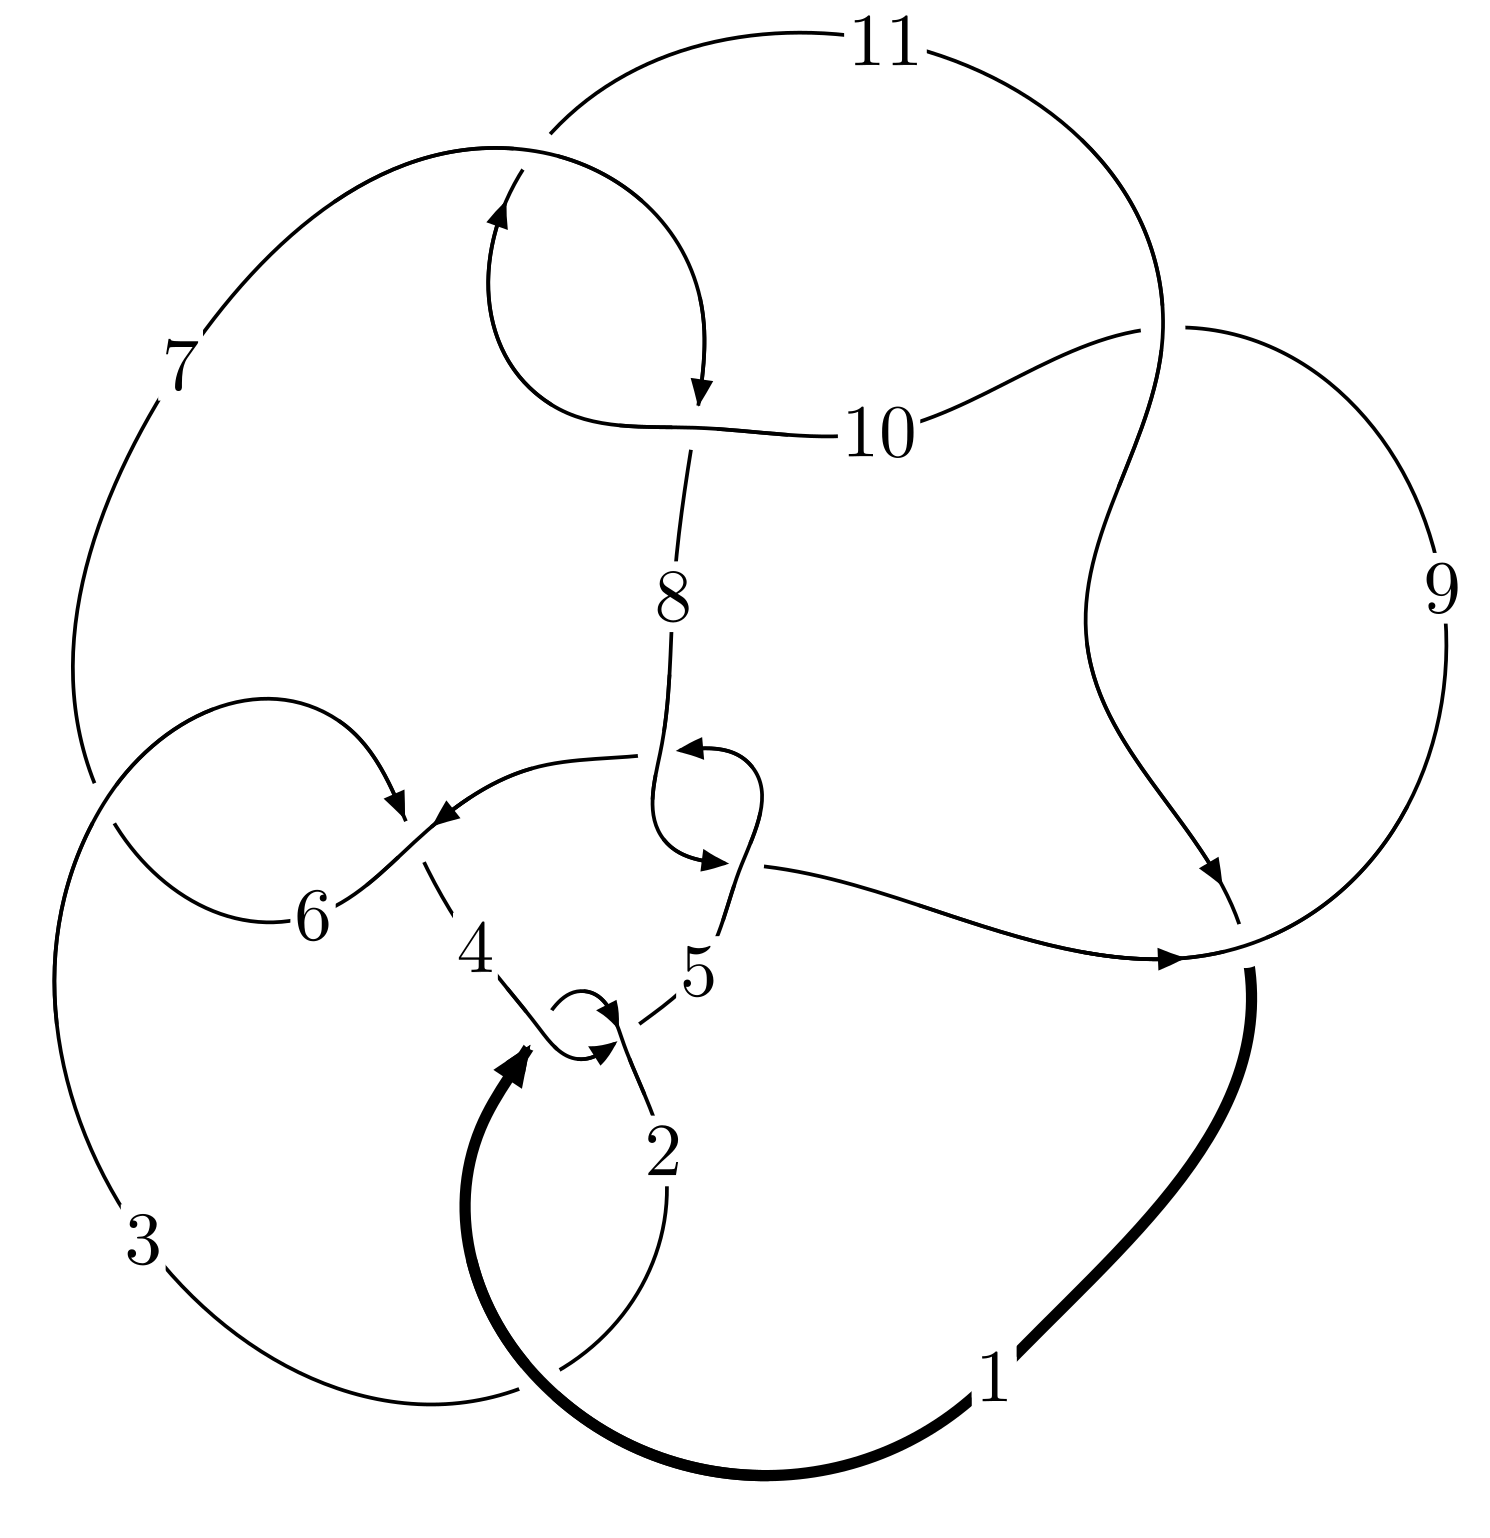
\includegraphics[width=112pt]{../../../GIT/diagram.site/Diagrams/png/266_11a_17.png}\\
\ \ \ A knot diagram\footnotemark}&
\allowdisplaybreaks
\textbf{Linearized knot diagam} \\
\cline{2-2}
 &
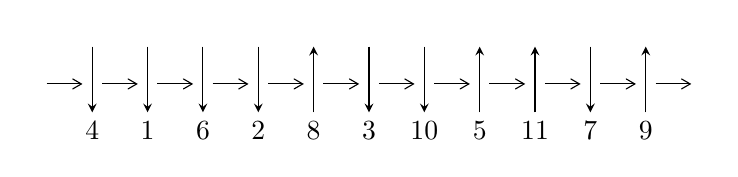
\begin{tikzpicture}[x=20pt, y=17pt]
	% nodes
	\node (C0) at (0, 0) {};
	\node (C1) at (1, 0) {};
	\node (C1U) at (1, +1) {};
	\node (C1D) at (1, -1) {4};

	\node (C2) at (2, 0) {};
	\node (C2U) at (2, +1) {};
	\node (C2D) at (2, -1) {1};

	\node (C3) at (3, 0) {};
	\node (C3U) at (3, +1) {};
	\node (C3D) at (3, -1) {6};

	\node (C4) at (4, 0) {};
	\node (C4U) at (4, +1) {};
	\node (C4D) at (4, -1) {2};

	\node (C5) at (5, 0) {};
	\node (C5U) at (5, +1) {};
	\node (C5D) at (5, -1) {8};

	\node (C6) at (6, 0) {};
	\node (C6U) at (6, +1) {};
	\node (C6D) at (6, -1) {3};

	\node (C7) at (7, 0) {};
	\node (C7U) at (7, +1) {};
	\node (C7D) at (7, -1) {10};

	\node (C8) at (8, 0) {};
	\node (C8U) at (8, +1) {};
	\node (C8D) at (8, -1) {5};

	\node (C9) at (9, 0) {};
	\node (C9U) at (9, +1) {};
	\node (C9D) at (9, -1) {11};

	\node (C10) at (10, 0) {};
	\node (C10U) at (10, +1) {};
	\node (C10D) at (10, -1) {7};

	\node (C11) at (11, 0) {};
	\node (C11U) at (11, +1) {};
	\node (C11D) at (11, -1) {9};
	\node (C12) at (12, 0) {};

	% arrows
	\draw[->,>={angle 60}]
	(C0) edge (C1) (C1) edge (C2) (C2) edge (C3) (C3) edge (C4) (C4) edge (C5) (C5) edge (C6) (C6) edge (C7) (C7) edge (C8) (C8) edge (C9) (C9) edge (C10) (C10) edge (C11) (C11) edge (C12) ;	\draw[->,>=stealth]
	(C1U) edge (C1D) (C2U) edge (C2D) (C3U) edge (C3D) (C4U) edge (C4D) (C5D) edge (C5U) (C6U) edge (C6D) (C7U) edge (C7D) (C8D) edge (C8U) (C9D) edge (C9U) (C10U) edge (C10D) (C11D) edge (C11U) ;
	\end{tikzpicture} \\
\hhline{~~} \\& 
\textbf{Solving Sequence} \\ \cline{2-2} 
 &
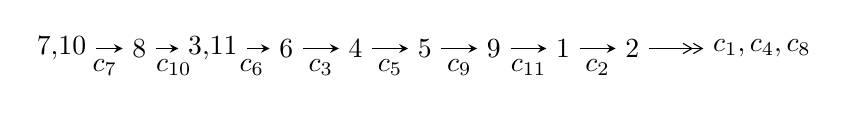
\begin{tikzpicture}[x=25pt, y=7pt]
	% node
	\node (A0) at (-1/8, 0) {7,10};
	\node (A1) at (1, 0) {8};
	\node (A2) at (33/16, 0) {3,11};
	\node (A3) at (25/8, 0) {6};
	\node (A4) at (33/8, 0) {4};
	\node (A5) at (41/8, 0) {5};
	\node (A6) at (49/8, 0) {9};
	\node (A7) at (57/8, 0) {1};
	\node (A8) at (65/8, 0) {2};
	\node (C1) at (1/2, -1) {$c_{7}$};
	\node (C2) at (3/2, -1) {$c_{10}$};
	\node (C3) at (21/8, -1) {$c_{6}$};
	\node (C4) at (29/8, -1) {$c_{3}$};
	\node (C5) at (37/8, -1) {$c_{5}$};
	\node (C6) at (45/8, -1) {$c_{9}$};
	\node (C7) at (53/8, -1) {$c_{11}$};
	\node (C8) at (61/8, -1) {$c_{2}$};
	\node (A9) at (10, 0) {$c_{1},c_{4},c_{8}$};

	% edge
	\draw[->,>=stealth]	
	(A0) edge (A1) (A1) edge (A2) (A2) edge (A3) (A3) edge (A4) (A4) edge (A5) (A5) edge (A6) (A6) edge (A7) (A7) edge (A8) ;
	\draw[->>,>={angle 60}]	
	(A8) edge (A9);
\end{tikzpicture} \\ 

\end{tabular} \\

\footnotetext{
The image of knot diagram is generated by the software ``\textbf{Draw programme}" developed by Andrew Bartholomew(\url{http://www.layer8.co.uk/maths/draw/index.htm\#Running-draw}), where we modified some parts for our purpose(\url{https://github.com/CATsTAILs/LinksPainter}).
}\phantom \\ \newline 
\centering \textbf{Ideals for irreducible components\footnotemark of $X_{\text{par}}$} 
 
\begin{align*}
I^u_{1}&=\langle 
-5.94953\times10^{22} u^{70}-2.28036\times10^{23} u^{69}+\cdots+2.14833\times10^{22} b-2.53129\times10^{22},\\
\phantom{I^u_{1}}&\phantom{= \langle  }9.79183\times10^{20} u^{70}+3.59725\times10^{22} u^{69}+\cdots+1.07416\times10^{22} a-8.03639\times10^{22},\;u^{71}+5 u^{70}+\cdots+16 u+1\rangle \\
I^u_{2}&=\langle 
-3 a^2 u+2 a^2-4 a u+7 b+5 a- u+10,\;a^3- a^2 u+2 a^2+3 a u- a+5 u,\;u^2- u+1\rangle \\
I^u_{3}&=\langle 
b,\;- u^3-2 u^2+a-2 u,\;u^4+u^3+u^2+1\rangle \\
\\
\end{align*}
\raggedright * 3 irreducible components of $\dim_{\mathbb{C}}=0$, with total 81 representations.\\
\footnotetext{All coefficients of polynomials are rational numbers. But the coefficients are sometimes approximated in decimal forms when there is not enough margin.}
\newpage
\renewcommand{\arraystretch}{1}
\centering \section*{I. $I^u_{1}= \langle -5.95\times10^{22} u^{70}-2.28\times10^{23} u^{69}+\cdots+2.15\times10^{22} b-2.53\times10^{22},\;9.79\times10^{20} u^{70}+3.60\times10^{22} u^{69}+\cdots+1.07\times10^{22} a-8.04\times10^{22},\;u^{71}+5 u^{70}+\cdots+16 u+1 \rangle$}
\flushleft \textbf{(i) Arc colorings}\\
\begin{tabular}{m{7pt} m{180pt} m{7pt} m{180pt} }
\flushright $a_{7}=$&$\begin{pmatrix}1\\0\end{pmatrix}$ \\
\flushright $a_{10}=$&$\begin{pmatrix}0\\u\end{pmatrix}$ \\
\flushright $a_{8}=$&$\begin{pmatrix}1\\u^2\end{pmatrix}$ \\
\flushright $a_{3}=$&$\begin{pmatrix}-0.0911577 u^{70}-3.34888 u^{69}+\cdots-37.5984 u+7.48153\\2.76938 u^{70}+10.6146 u^{69}+\cdots+12.1316 u+1.17826\end{pmatrix}$ \\
\flushright $a_{11}=$&$\begin{pmatrix}- u\\u\end{pmatrix}$ \\
\flushright $a_{6}=$&$\begin{pmatrix}4.02087 u^{70}+14.8653 u^{69}+\cdots+22.0738 u-2.91262\\-2.20047 u^{70}-6.62609 u^{69}+\cdots+2.44001 u-0.00293030\end{pmatrix}$ \\
\flushright $a_{4}=$&$\begin{pmatrix}-4.91020 u^{70}-23.2455 u^{69}+\cdots-75.9832 u+7.34450\\5.57560 u^{70}+18.7187 u^{69}+\cdots-10.4341 u-0.354339\end{pmatrix}$ \\
\flushright $a_{5}=$&$\begin{pmatrix}8.28715 u^{70}+36.7438 u^{69}+\cdots+99.4370 u+2.32932\\-8.83708 u^{70}-30.6563 u^{69}+\cdots-10.5783 u-0.549932\end{pmatrix}$ \\
\flushright $a_{9}=$&$\begin{pmatrix}- u^3\\u^3+u\end{pmatrix}$ \\
\flushright $a_{1}=$&$\begin{pmatrix}- u^5- u\\u^5+u^3+u\end{pmatrix}$ \\
\flushright $a_{2}=$&$\begin{pmatrix}1.84442 u^{70}+6.91573 u^{69}+\cdots+0.676442 u+9.99389\\0.311963 u^{70}+1.82295 u^{69}+\cdots+10.8155 u+1.16954\end{pmatrix}$\\ \flushright $a_{2}=$&$\begin{pmatrix}1.84442 u^{70}+6.91573 u^{69}+\cdots+0.676442 u+9.99389\\0.311963 u^{70}+1.82295 u^{69}+\cdots+10.8155 u+1.16954\end{pmatrix}$\\&\end{tabular}
\flushleft \textbf{(ii) Obstruction class $= -1$}\\~\\
\flushleft \textbf{(iii) Cusp Shapes $= \frac{14007707892704021288689}{10741642455012495551282} u^{70}+\frac{52903988225635842251755}{10741642455012495551282} u^{69}+\cdots+\frac{406218822228831882964265}{10741642455012495551282} u-\frac{31847081302722889929098}{5370821227506247775641}$}\\~\\
\newpage\renewcommand{\arraystretch}{1}
\flushleft \textbf{(iv) u-Polynomials at the component}\newline \\
\begin{tabular}{m{50pt}|m{274pt}}
Crossings & \hspace{64pt}u-Polynomials at each crossing \\
\hline $$\begin{aligned}c_{1},c_{4}\end{aligned}$$&$\begin{aligned}
&u^{71}-7 u^{70}+\cdots-19 u+1
\end{aligned}$\\
\hline $$\begin{aligned}c_{2}\end{aligned}$$&$\begin{aligned}
&u^{71}+35 u^{70}+\cdots+91 u+1
\end{aligned}$\\
\hline $$\begin{aligned}c_{3},c_{6}\end{aligned}$$&$\begin{aligned}
&u^{71}-3 u^{70}+\cdots-72 u+16
\end{aligned}$\\
\hline $$\begin{aligned}c_{5},c_{8}\end{aligned}$$&$\begin{aligned}
&u^{71}+2 u^{70}+\cdots+224 u+64
\end{aligned}$\\
\hline $$\begin{aligned}c_{7},c_{10}\end{aligned}$$&$\begin{aligned}
&u^{71}-5 u^{70}+\cdots+16 u-1
\end{aligned}$\\
\hline $$\begin{aligned}c_{9},c_{11}\end{aligned}$$&$\begin{aligned}
&u^{71}-23 u^{70}+\cdots+246 u+1
\end{aligned}$\\
\hline
\end{tabular}\\~\\
\newpage\renewcommand{\arraystretch}{1}
\flushleft \textbf{(v) Riley Polynomials at the component}\newline \\
\begin{tabular}{m{50pt}|m{274pt}}
Crossings & \hspace{64pt}Riley Polynomials at each crossing \\
\hline $$\begin{aligned}c_{1},c_{4}\end{aligned}$$&$\begin{aligned}
&y^{71}-35 y^{70}+\cdots+91 y-1
\end{aligned}$\\
\hline $$\begin{aligned}c_{2}\end{aligned}$$&$\begin{aligned}
&y^{71}+9 y^{70}+\cdots+3279 y-1
\end{aligned}$\\
\hline $$\begin{aligned}c_{3},c_{6}\end{aligned}$$&$\begin{aligned}
&y^{71}+33 y^{70}+\cdots-4800 y-256
\end{aligned}$\\
\hline $$\begin{aligned}c_{5},c_{8}\end{aligned}$$&$\begin{aligned}
&y^{71}+40 y^{70}+\cdots-39936 y-4096
\end{aligned}$\\
\hline $$\begin{aligned}c_{7},c_{10}\end{aligned}$$&$\begin{aligned}
&y^{71}+23 y^{70}+\cdots+246 y-1
\end{aligned}$\\
\hline $$\begin{aligned}c_{9},c_{11}\end{aligned}$$&$\begin{aligned}
&y^{71}+55 y^{70}+\cdots+62490 y-1
\end{aligned}$\\
\hline
\end{tabular}\\~\\
\newpage\flushleft \textbf{(vi) Complex Volumes and Cusp Shapes}
$$\begin{array}{c|c|c}  
\text{Solutions to }I^u_{1}& \I (\text{vol} + \sqrt{-1}CS) & \text{Cusp shape}\\
 \hline 
\begin{aligned}
u &= \phantom{-}0.469540 + 0.901499 I \\
a &= -2.34185 + 1.83693 I \\
b &= -0.440954 - 0.146276 I\end{aligned}
 & -1.31688 - 1.88106 I & -31.3196 + 4.6871 I \\ \hline\begin{aligned}
u &= \phantom{-}0.469540 - 0.901499 I \\
a &= -2.34185 - 1.83693 I \\
b &= -0.440954 + 0.146276 I\end{aligned}
 & -1.31688 + 1.88106 I & -31.3196 - 4.6871 I \\ \hline\begin{aligned}
u &= \phantom{-}0.703653 + 0.685371 I \\
a &= -0.410681 + 0.049842 I \\
b &= -0.285900 + 0.818152 I\end{aligned}
 & \phantom{-}0.185937 - 1.104380 I & -1.16040 + 2.40265 I \\ \hline\begin{aligned}
u &= \phantom{-}0.703653 - 0.685371 I \\
a &= -0.410681 - 0.049842 I \\
b &= -0.285900 - 0.818152 I\end{aligned}
 & \phantom{-}0.185937 + 1.104380 I & -1.16040 - 2.40265 I \\ \hline\begin{aligned}
u &= -0.066834 + 0.978657 I \\
a &= -0.76286 - 2.56276 I \\
b &= -0.149859 + 1.246530 I\end{aligned}
 & \phantom{-}5.52736 - 0.93567 I & \phantom{-}4.64414 + 2.41235 I \\ \hline\begin{aligned}
u &= -0.066834 - 0.978657 I \\
a &= -0.76286 + 2.56276 I \\
b &= -0.149859 - 1.246530 I\end{aligned}
 & \phantom{-}5.52736 + 0.93567 I & \phantom{-}4.64414 - 2.41235 I \\ \hline\begin{aligned}
u &= \phantom{-}0.199067 + 1.029270 I \\
a &= \phantom{-}0.844886 - 0.722840 I \\
b &= -0.903463 + 0.396432 I\end{aligned}
 & -0.16872 - 3.86400 I & \phantom{-0.000000 -}0. + 6.04330 I \\ \hline\begin{aligned}
u &= \phantom{-}0.199067 - 1.029270 I \\
a &= \phantom{-}0.844886 + 0.722840 I \\
b &= -0.903463 - 0.396432 I\end{aligned}
 & -0.16872 + 3.86400 I & \phantom{-0.000000 } 0. - 6.04330 I \\ \hline\begin{aligned}
u &= \phantom{-}0.228246 + 0.913383 I \\
a &= -0.23825 + 3.38061 I \\
b &= -0.223038 - 0.668311 I\end{aligned}
 & -1.01028 - 1.75385 I & \phantom{-}0.38756 + 7.39042 I \\ \hline\begin{aligned}
u &= \phantom{-}0.228246 - 0.913383 I \\
a &= -0.23825 - 3.38061 I \\
b &= -0.223038 + 0.668311 I\end{aligned}
 & -1.01028 + 1.75385 I & \phantom{-}0.38756 - 7.39042 I\\
 \hline 
 \end{array}$$\newpage$$\begin{array}{c|c|c}  
\text{Solutions to }I^u_{1}& \I (\text{vol} + \sqrt{-1}CS) & \text{Cusp shape}\\
 \hline 
\begin{aligned}
u &= -0.644181 + 0.840361 I \\
a &= -1.06472 - 1.25613 I \\
b &= \phantom{-}0.21087 + 1.49010 I\end{aligned}
 & \phantom{-}2.18680 - 0.67401 I & \phantom{-0.000000 } 0 \\ \hline\begin{aligned}
u &= -0.644181 - 0.840361 I \\
a &= -1.06472 + 1.25613 I \\
b &= \phantom{-}0.21087 - 1.49010 I\end{aligned}
 & \phantom{-}2.18680 + 0.67401 I & \phantom{-0.000000 } 0 \\ \hline\begin{aligned}
u &= -0.170132 + 0.914729 I \\
a &= \phantom{-}1.00662 + 2.47886 I \\
b &= \phantom{-}0.419700 - 1.267450 I\end{aligned}
 & \phantom{-}4.39627 + 4.60339 I & \phantom{-}3.32762 - 2.73353 I \\ \hline\begin{aligned}
u &= -0.170132 - 0.914729 I \\
a &= \phantom{-}1.00662 - 2.47886 I \\
b &= \phantom{-}0.419700 + 1.267450 I\end{aligned}
 & \phantom{-}4.39627 - 4.60339 I & \phantom{-}3.32762 + 2.73353 I \\ \hline\begin{aligned}
u &= -0.836021 + 0.673858 I \\
a &= \phantom{-}0.109662 - 0.484018 I \\
b &= \phantom{-}0.672234 + 1.164290 I\end{aligned}
 & -2.39090 - 4.48377 I & \phantom{-0.000000 } 0 \\ \hline\begin{aligned}
u &= -0.836021 - 0.673858 I \\
a &= \phantom{-}0.109662 + 0.484018 I \\
b &= \phantom{-}0.672234 - 1.164290 I\end{aligned}
 & -2.39090 + 4.48377 I & \phantom{-0.000000 } 0 \\ \hline\begin{aligned}
u &= \phantom{-}0.682896 + 0.834787 I \\
a &= \phantom{-}1.99324 - 0.92672 I \\
b &= \phantom{-}0.617687 + 0.601618 I\end{aligned}
 & -3.08372 - 1.52053 I & \phantom{-0.000000 } 0 \\ \hline\begin{aligned}
u &= \phantom{-}0.682896 - 0.834787 I \\
a &= \phantom{-}1.99324 + 0.92672 I \\
b &= \phantom{-}0.617687 - 0.601618 I\end{aligned}
 & -3.08372 + 1.52053 I & \phantom{-0.000000 } 0 \\ \hline\begin{aligned}
u &= -0.832336 + 0.724886 I \\
a &= -0.670615 - 0.613985 I \\
b &= -1.075770 + 0.627927 I\end{aligned}
 & -6.99333 - 3.33145 I & \phantom{-0.000000 } 0 \\ \hline\begin{aligned}
u &= -0.832336 - 0.724886 I \\
a &= -0.670615 + 0.613985 I \\
b &= -1.075770 - 0.627927 I\end{aligned}
 & -6.99333 + 3.33145 I & \phantom{-0.000000 } 0\\
 \hline 
 \end{array}$$\newpage$$\begin{array}{c|c|c}  
\text{Solutions to }I^u_{1}& \I (\text{vol} + \sqrt{-1}CS) & \text{Cusp shape}\\
 \hline 
\begin{aligned}
u &= \phantom{-}0.140143 + 1.101750 I \\
a &= -0.13050 - 2.45616 I \\
b &= \phantom{-}0.426470 + 1.144810 I\end{aligned}
 & \phantom{-}4.31628 - 4.18567 I & \phantom{-0.000000 } 0 \\ \hline\begin{aligned}
u &= \phantom{-}0.140143 - 1.101750 I \\
a &= -0.13050 + 2.45616 I \\
b &= \phantom{-}0.426470 - 1.144810 I\end{aligned}
 & \phantom{-}4.31628 + 4.18567 I & \phantom{-0.000000 } 0 \\ \hline\begin{aligned}
u &= -0.780059 + 0.792579 I \\
a &= \phantom{-}0.408945 + 0.711158 I \\
b &= \phantom{-}1.044280 - 0.406192 I\end{aligned}
 & -4.75730 + 1.60644 I & \phantom{-0.000000 } 0 \\ \hline\begin{aligned}
u &= -0.780059 - 0.792579 I \\
a &= \phantom{-}0.408945 - 0.711158 I \\
b &= \phantom{-}1.044280 + 0.406192 I\end{aligned}
 & -4.75730 - 1.60644 I & \phantom{-0.000000 } 0 \\ \hline\begin{aligned}
u &= -0.649958 + 0.906097 I \\
a &= \phantom{-}1.16875 + 1.58162 I \\
b &= \phantom{-}0.08760 - 1.49800 I\end{aligned}
 & \phantom{-}2.40563 + 5.71061 I & \phantom{-0.000000 } 0 \\ \hline\begin{aligned}
u &= -0.649958 - 0.906097 I \\
a &= \phantom{-}1.16875 - 1.58162 I \\
b &= \phantom{-}0.08760 + 1.49800 I\end{aligned}
 & \phantom{-}2.40563 - 5.71061 I & \phantom{-0.000000 } 0 \\ \hline\begin{aligned}
u &= -0.819648 + 0.758949 I \\
a &= -0.202166 + 0.947127 I \\
b &= -0.555895 - 1.022590 I\end{aligned}
 & -7.65318 - 0.42476 I & \phantom{-0.000000 } 0 \\ \hline\begin{aligned}
u &= -0.819648 - 0.758949 I \\
a &= -0.202166 - 0.947127 I \\
b &= -0.555895 + 1.022590 I\end{aligned}
 & -7.65318 + 0.42476 I & \phantom{-0.000000 } 0 \\ \hline\begin{aligned}
u &= -0.892301 + 0.672315 I \\
a &= -0.295771 + 0.358689 I \\
b &= -0.776807 - 1.153330 I\end{aligned}
 & -5.27544 - 10.02070 I & \phantom{-0.000000 } 0 \\ \hline\begin{aligned}
u &= -0.892301 - 0.672315 I \\
a &= -0.295771 - 0.358689 I \\
b &= -0.776807 + 1.153330 I\end{aligned}
 & -5.27544 + 10.02070 I & \phantom{-0.000000 } 0\\
 \hline 
 \end{array}$$\newpage$$\begin{array}{c|c|c}  
\text{Solutions to }I^u_{1}& \I (\text{vol} + \sqrt{-1}CS) & \text{Cusp shape}\\
 \hline 
\begin{aligned}
u &= \phantom{-}0.809277 + 0.772791 I \\
a &= \phantom{-}0.335402 - 0.318821 I \\
b &= \phantom{-}0.572324 - 0.999549 I\end{aligned}
 & -1.88125 + 3.19322 I & \phantom{-0.000000 } 0 \\ \hline\begin{aligned}
u &= \phantom{-}0.809277 - 0.772791 I \\
a &= \phantom{-}0.335402 + 0.318821 I \\
b &= \phantom{-}0.572324 + 0.999549 I\end{aligned}
 & -1.88125 - 3.19322 I & \phantom{-0.000000 } 0 \\ \hline\begin{aligned}
u &= \phantom{-}0.684814 + 0.898763 I \\
a &= \phantom{-}0.736483 - 0.552503 I \\
b &= \phantom{-}0.770057 - 0.536295 I\end{aligned}
 & -2.88221 - 3.75765 I & \phantom{-0.000000 } 0 \\ \hline\begin{aligned}
u &= \phantom{-}0.684814 - 0.898763 I \\
a &= \phantom{-}0.736483 + 0.552503 I \\
b &= \phantom{-}0.770057 + 0.536295 I\end{aligned}
 & -2.88221 + 3.75765 I & \phantom{-0.000000 } 0 \\ \hline\begin{aligned}
u &= \phantom{-}0.063523 + 0.862035 I \\
a &= -0.858693 + 0.495191 I \\
b &= \phantom{-}0.869259 + 0.100924 I\end{aligned}
 & \phantom{-}0.623561 - 0.155557 I & \phantom{-}0.0220175 - 0.0069970 I \\ \hline\begin{aligned}
u &= \phantom{-}0.063523 - 0.862035 I \\
a &= -0.858693 - 0.495191 I \\
b &= \phantom{-}0.869259 - 0.100924 I\end{aligned}
 & \phantom{-}0.623561 + 0.155557 I & \phantom{-}0.0220175 + 0.0069970 I \\ \hline\begin{aligned}
u &= \phantom{-}0.825029 + 0.180514 I \\
a &= -0.358331 + 0.374895 I \\
b &= -0.613697 - 1.017340 I\end{aligned}
 & -2.42985 - 6.27823 I & -7.32031 + 6.32359 I \\ \hline\begin{aligned}
u &= \phantom{-}0.825029 - 0.180514 I \\
a &= -0.358331 - 0.374895 I \\
b &= -0.613697 + 1.017340 I\end{aligned}
 & -2.42985 + 6.27823 I & -7.32031 - 6.32359 I \\ \hline\begin{aligned}
u &= \phantom{-}0.190670 + 1.155730 I \\
a &= \phantom{-}0.01366 + 2.28563 I \\
b &= -0.628836 - 1.153550 I\end{aligned}
 & \phantom{-}2.15092 - 9.48353 I & \phantom{-0.000000 } 0 \\ \hline\begin{aligned}
u &= \phantom{-}0.190670 - 1.155730 I \\
a &= \phantom{-}0.01366 - 2.28563 I \\
b &= -0.628836 + 1.153550 I\end{aligned}
 & \phantom{-}2.15092 + 9.48353 I & \phantom{-0.000000 } 0\\
 \hline 
 \end{array}$$\newpage$$\begin{array}{c|c|c}  
\text{Solutions to }I^u_{1}& \I (\text{vol} + \sqrt{-1}CS) & \text{Cusp shape}\\
 \hline 
\begin{aligned}
u &= \phantom{-}0.532399 + 1.050880 I \\
a &= -1.16792 + 1.12279 I \\
b &= \phantom{-}0.139051 - 0.972541 I\end{aligned}
 & \phantom{-}1.97142 - 2.68154 I & \phantom{-0.000000 } 0 \\ \hline\begin{aligned}
u &= \phantom{-}0.532399 - 1.050880 I \\
a &= -1.16792 - 1.12279 I \\
b &= \phantom{-}0.139051 + 0.972541 I\end{aligned}
 & \phantom{-}1.97142 + 2.68154 I & \phantom{-0.000000 } 0 \\ \hline\begin{aligned}
u &= \phantom{-}0.682581 + 0.973399 I \\
a &= -1.55596 + 1.01812 I \\
b &= -0.423358 - 0.977979 I\end{aligned}
 & \phantom{-}1.01578 - 4.23738 I & \phantom{-0.000000 } 0 \\ \hline\begin{aligned}
u &= \phantom{-}0.682581 - 0.973399 I \\
a &= -1.55596 - 1.01812 I \\
b &= -0.423358 + 0.977979 I\end{aligned}
 & \phantom{-}1.01578 + 4.23738 I & \phantom{-0.000000 } 0 \\ \hline\begin{aligned}
u &= -0.737484 + 0.947027 I \\
a &= -0.255221 + 0.689415 I \\
b &= \phantom{-}1.108830 + 0.298809 I\end{aligned}
 & -4.27963 + 4.12596 I & \phantom{-0.000000 } 0 \\ \hline\begin{aligned}
u &= -0.737484 - 0.947027 I \\
a &= -0.255221 - 0.689415 I \\
b &= \phantom{-}1.108830 - 0.298809 I\end{aligned}
 & -4.27963 - 4.12596 I & \phantom{-0.000000 } 0 \\ \hline\begin{aligned}
u &= \phantom{-}0.449989 + 1.115620 I \\
a &= \phantom{-}1.04346 - 0.97703 I \\
b &= -0.474923 + 1.017330 I\end{aligned}
 & \phantom{-}0.54346 + 1.75236 I & \phantom{-0.000000 } 0 \\ \hline\begin{aligned}
u &= \phantom{-}0.449989 - 1.115620 I \\
a &= \phantom{-}1.04346 + 0.97703 I \\
b &= -0.474923 - 1.017330 I\end{aligned}
 & \phantom{-}0.54346 - 1.75236 I & \phantom{-0.000000 } 0 \\ \hline\begin{aligned}
u &= \phantom{-}0.435093 + 0.655870 I \\
a &= -0.421928 - 0.262313 I \\
b &= \phantom{-}0.013074 + 0.389178 I\end{aligned}
 & \phantom{-}0.058062 - 1.373770 I & \phantom{-}0.54762 + 4.59641 I \\ \hline\begin{aligned}
u &= \phantom{-}0.435093 - 0.655870 I \\
a &= -0.421928 + 0.262313 I \\
b &= \phantom{-}0.013074 - 0.389178 I\end{aligned}
 & \phantom{-}0.058062 + 1.373770 I & \phantom{-}0.54762 - 4.59641 I\\
 \hline 
 \end{array}$$\newpage$$\begin{array}{c|c|c}  
\text{Solutions to }I^u_{1}& \I (\text{vol} + \sqrt{-1}CS) & \text{Cusp shape}\\
 \hline 
\begin{aligned}
u &= \phantom{-}0.750193 + 0.971797 I \\
a &= \phantom{-}1.56758 - 0.87634 I \\
b &= \phantom{-}0.625386 + 1.066570 I\end{aligned}
 & -1.26633 - 9.05370 I & \phantom{-0.000000 } 0 \\ \hline\begin{aligned}
u &= \phantom{-}0.750193 - 0.971797 I \\
a &= \phantom{-}1.56758 + 0.87634 I \\
b &= \phantom{-}0.625386 - 1.066570 I\end{aligned}
 & -1.26633 + 9.05370 I & \phantom{-0.000000 } 0 \\ \hline\begin{aligned}
u &= -0.751292 + 0.980442 I \\
a &= -1.30409 - 1.91476 I \\
b &= -0.474824 + 1.073280 I\end{aligned}
 & -6.97127 + 6.31431 I & \phantom{-0.000000 } 0 \\ \hline\begin{aligned}
u &= -0.751292 - 0.980442 I \\
a &= -1.30409 + 1.91476 I \\
b &= -0.474824 - 1.073280 I\end{aligned}
 & -6.97127 - 6.31431 I & \phantom{-0.000000 } 0 \\ \hline\begin{aligned}
u &= -0.888822 + 0.861156 I \\
a &= -0.420743 - 0.227554 I \\
b &= -0.503579 + 0.631395 I\end{aligned}
 & -8.93127 + 3.93572 I & \phantom{-0.000000 } 0 \\ \hline\begin{aligned}
u &= -0.888822 - 0.861156 I \\
a &= -0.420743 + 0.227554 I \\
b &= -0.503579 - 0.631395 I\end{aligned}
 & -8.93127 - 3.93572 I & \phantom{-0.000000 } 0 \\ \hline\begin{aligned}
u &= -0.745302 + 1.004020 I \\
a &= \phantom{-}0.429820 - 0.617085 I \\
b &= -1.133830 - 0.574421 I\end{aligned}
 & -6.13711 + 9.23592 I & \phantom{-0.000000 } 0 \\ \hline\begin{aligned}
u &= -0.745302 - 1.004020 I \\
a &= \phantom{-}0.429820 + 0.617085 I \\
b &= -1.133830 + 0.574421 I\end{aligned}
 & -6.13711 - 9.23592 I & \phantom{-0.000000 } 0 \\ \hline\begin{aligned}
u &= -0.728006 + 1.029620 I \\
a &= \phantom{-}1.30483 + 1.76760 I \\
b &= \phantom{-}0.653700 - 1.243700 I\end{aligned}
 & -1.30783 + 10.33650 I & \phantom{-0.000000 } 0 \\ \hline\begin{aligned}
u &= -0.728006 - 1.029620 I \\
a &= \phantom{-}1.30483 - 1.76760 I \\
b &= \phantom{-}0.653700 + 1.243700 I\end{aligned}
 & -1.30783 - 10.33650 I & \phantom{-0.000000 } 0\\
 \hline 
 \end{array}$$\newpage$$\begin{array}{c|c|c}  
\text{Solutions to }I^u_{1}& \I (\text{vol} + \sqrt{-1}CS) & \text{Cusp shape}\\
 \hline 
\begin{aligned}
u &= \phantom{-}0.665608 + 0.272736 I \\
a &= \phantom{-}0.030085 - 0.514045 I \\
b &= \phantom{-}0.406144 + 0.846985 I\end{aligned}
 & -0.11266 - 1.79745 I & -3.68305 + 3.00636 I \\ \hline\begin{aligned}
u &= \phantom{-}0.665608 - 0.272736 I \\
a &= \phantom{-}0.030085 + 0.514045 I \\
b &= \phantom{-}0.406144 - 0.846985 I\end{aligned}
 & -0.11266 + 1.79745 I & -3.68305 - 3.00636 I \\ \hline\begin{aligned}
u &= -0.852550 + 0.956405 I \\
a &= \phantom{-}0.320716 - 0.242205 I \\
b &= -0.414388 - 0.586515 I\end{aligned}
 & -8.63777 + 2.49143 I & \phantom{-0.000000 } 0 \\ \hline\begin{aligned}
u &= -0.852550 - 0.956405 I \\
a &= \phantom{-}0.320716 + 0.242205 I \\
b &= -0.414388 + 0.586515 I\end{aligned}
 & -8.63777 - 2.49143 I & \phantom{-0.000000 } 0 \\ \hline\begin{aligned}
u &= -0.749415 + 1.052960 I \\
a &= -1.33912 - 1.71674 I \\
b &= -0.77993 + 1.20298 I\end{aligned}
 & -4.0986 + 16.1013 I & \phantom{-0.000000 } 0 \\ \hline\begin{aligned}
u &= -0.749415 - 1.052960 I \\
a &= -1.33912 + 1.71674 I \\
b &= -0.77993 - 1.20298 I\end{aligned}
 & -4.0986 - 16.1013 I & \phantom{-0.000000 } 0 \\ \hline\begin{aligned}
u &= \phantom{-}0.633866 + 0.064239 I \\
a &= -0.737841 - 1.003620 I \\
b &= -0.712988 + 0.613513 I\end{aligned}
 & -3.67287 - 1.17347 I & -10.32734 + 0.68526 I \\ \hline\begin{aligned}
u &= \phantom{-}0.633866 - 0.064239 I \\
a &= -0.737841 + 1.003620 I \\
b &= -0.712988 - 0.613513 I\end{aligned}
 & -3.67287 + 1.17347 I & -10.32734 - 0.68526 I \\ \hline\begin{aligned}
u &= -0.470621 + 0.142712 I \\
a &= -0.309496 + 0.762972 I \\
b &= \phantom{-}0.176109 + 1.095200 I\end{aligned}
 & \phantom{-}2.07880 - 2.37441 I & -0.70861 + 4.00251 I \\ \hline\begin{aligned}
u &= -0.470621 - 0.142712 I \\
a &= -0.309496 - 0.762972 I \\
b &= \phantom{-}0.176109 - 1.095200 I\end{aligned}
 & \phantom{-}2.07880 + 2.37441 I & -0.70861 - 4.00251 I\\
 \hline 
 \end{array}$$\newpage$$\begin{array}{c|c|c}  
\text{Solutions to }I^u_{1}& \I (\text{vol} + \sqrt{-1}CS) & \text{Cusp shape}\\
 \hline 
\begin{aligned}
u &= -0.0632515\phantom{ +0.000000I} \\
a &= \phantom{-}10.0652\phantom{ +0.000000I} \\
b &= \phantom{-}0.518539\phantom{ +0.000000I}\end{aligned}
 & -1.19409\phantom{ +0.000000I} & -8.46120\phantom{ +0.000000I}\\
 \hline 
 \end{array}$$\newpage\newpage\renewcommand{\arraystretch}{1}
\centering \section*{II. $I^u_{2}= \langle -3 a^2 u+2 a^2-4 a u+7 b+5 a- u+10,\;a^3- a^2 u+2 a^2+3 a u- a+5 u,\;u^2- u+1 \rangle$}
\flushleft \textbf{(i) Arc colorings}\\
\begin{tabular}{m{7pt} m{180pt} m{7pt} m{180pt} }
\flushright $a_{7}=$&$\begin{pmatrix}1\\0\end{pmatrix}$ \\
\flushright $a_{10}=$&$\begin{pmatrix}0\\u\end{pmatrix}$ \\
\flushright $a_{8}=$&$\begin{pmatrix}1\\u-1\end{pmatrix}$ \\
\flushright $a_{3}=$&$\begin{pmatrix}a\\\frac{3}{7} a^2 u+\frac{4}{7} a u+\cdots-\frac{5}{7} a-\frac{10}{7}\end{pmatrix}$ \\
\flushright $a_{11}=$&$\begin{pmatrix}- u\\u\end{pmatrix}$ \\
\flushright $a_{6}=$&$\begin{pmatrix}\frac{1}{7} a^2 u-\frac{1}{7} a u+\cdots+\frac{3}{7} a-\frac{8}{7}\\\frac{4}{7} a^2 u+\frac{3}{7} a u+\cdots-\frac{2}{7} a+\frac{3}{7}\end{pmatrix}$ \\
\flushright $a_{4}=$&$\begin{pmatrix}\frac{3}{7} a^2 u-\frac{3}{7} a u+\cdots+\frac{2}{7} a-\frac{10}{7}\\\frac{1}{7} a^2 u-\frac{1}{7} a u+\cdots+\frac{3}{7} a+\frac{6}{7}\end{pmatrix}$ \\
\flushright $a_{5}=$&$\begin{pmatrix}\frac{1}{7} a^2 u-\frac{1}{7} a u+\cdots+\frac{3}{7} a-\frac{8}{7}\\\frac{4}{7} a^2 u+\frac{3}{7} a u+\cdots-\frac{2}{7} a+\frac{3}{7}\end{pmatrix}$ \\
\flushright $a_{9}=$&$\begin{pmatrix}1\\u-1\end{pmatrix}$ \\
\flushright $a_{1}=$&$\begin{pmatrix}-1\\0\end{pmatrix}$ \\
\flushright $a_{2}=$&$\begin{pmatrix}\frac{3}{7} a^2 u+\frac{4}{7} a u+\cdots+\frac{2}{7} a-\frac{10}{7}\\\frac{3}{7} a^2 u+\frac{4}{7} a u+\cdots-\frac{5}{7} a-\frac{10}{7}\end{pmatrix}$\\ \flushright $a_{2}=$&$\begin{pmatrix}\frac{3}{7} a^2 u+\frac{4}{7} a u+\cdots+\frac{2}{7} a-\frac{10}{7}\\\frac{3}{7} a^2 u+\frac{4}{7} a u+\cdots-\frac{5}{7} a-\frac{10}{7}\end{pmatrix}$\\&\end{tabular}
\flushleft \textbf{(ii) Obstruction class $= 1$}\\~\\
\flushleft \textbf{(iii) Cusp Shapes $= \frac{18}{7} a^2 u+\frac{2}{7} a^2-\frac{4}{7} a u+\frac{19}{7} a+\frac{62}{7} u-\frac{67}{7}$}\\~\\
\newpage\renewcommand{\arraystretch}{1}
\flushleft \textbf{(iv) u-Polynomials at the component}\newline \\
\begin{tabular}{m{50pt}|m{274pt}}
Crossings & \hspace{64pt}u-Polynomials at each crossing \\
\hline $$\begin{aligned}c_{1}\end{aligned}$$&$\begin{aligned}
&(u^3+u^2-1)^2
\end{aligned}$\\
\hline $$\begin{aligned}c_{2},c_{6}\end{aligned}$$&$\begin{aligned}
&(u^3+u^2+2 u+1)^2
\end{aligned}$\\
\hline $$\begin{aligned}c_{3}\end{aligned}$$&$\begin{aligned}
&(u^3- u^2+2 u-1)^2
\end{aligned}$\\
\hline $$\begin{aligned}c_{4}\end{aligned}$$&$\begin{aligned}
&(u^3- u^2+1)^2
\end{aligned}$\\
\hline $$\begin{aligned}c_{5},c_{8}\end{aligned}$$&$\begin{aligned}
&u^6
\end{aligned}$\\
\hline $$\begin{aligned}c_{7},c_{11}\end{aligned}$$&$\begin{aligned}
&(u^2- u+1)^3
\end{aligned}$\\
\hline $$\begin{aligned}c_{9},c_{10}\end{aligned}$$&$\begin{aligned}
&(u^2+u+1)^3
\end{aligned}$\\
\hline
\end{tabular}\\~\\
\newpage\renewcommand{\arraystretch}{1}
\flushleft \textbf{(v) Riley Polynomials at the component}\newline \\
\begin{tabular}{m{50pt}|m{274pt}}
Crossings & \hspace{64pt}Riley Polynomials at each crossing \\
\hline $$\begin{aligned}c_{1},c_{4}\end{aligned}$$&$\begin{aligned}
&(y^3- y^2+2 y-1)^2
\end{aligned}$\\
\hline $$\begin{aligned}c_{2},c_{3},c_{6}\end{aligned}$$&$\begin{aligned}
&(y^3+3 y^2+2 y-1)^2
\end{aligned}$\\
\hline $$\begin{aligned}c_{5},c_{8}\end{aligned}$$&$\begin{aligned}
&y^6
\end{aligned}$\\
\hline $$\begin{aligned}c_{7},c_{9},c_{10}\\c_{11}\end{aligned}$$&$\begin{aligned}
&(y^2+y+1)^3
\end{aligned}$\\
\hline
\end{tabular}\\~\\
\newpage\flushleft \textbf{(vi) Complex Volumes and Cusp Shapes}
$$\begin{array}{c|c|c}  
\text{Solutions to }I^u_{2}& \I (\text{vol} + \sqrt{-1}CS) & \text{Cusp shape}\\
 \hline 
\begin{aligned}
u &= \phantom{-}0.500000 + 0.866025 I \\
a &= -1.46996 + 0.49350 I \\
b &= -0.569840\phantom{ +0.000000I}\end{aligned}
 & -1.11345 - 2.02988 I & -2.22484 + 11.58609 I \\ \hline\begin{aligned}
u &= \phantom{-}0.500000 + 0.866025 I \\
a &= \phantom{-}1.11700 - 1.21217 I \\
b &= -0.215080 + 1.307140 I\end{aligned}
 & \phantom{-}3.02413 + 0.79824 I & \phantom{-}2.65209 - 0.57512 I \\ \hline\begin{aligned}
u &= \phantom{-}0.500000 + 0.866025 I \\
a &= -1.14704 + 1.58470 I \\
b &= -0.215080 - 1.307140 I\end{aligned}
 & \phantom{-}3.02413 - 4.85801 I & -0.92725 + 3.71146 I \\ \hline\begin{aligned}
u &= \phantom{-}0.500000 - 0.866025 I \\
a &= -1.46996 - 0.49350 I \\
b &= -0.569840\phantom{ +0.000000I}\end{aligned}
 & -1.11345 + 2.02988 I & -2.22484 - 11.58609 I \\ \hline\begin{aligned}
u &= \phantom{-}0.500000 - 0.866025 I \\
a &= \phantom{-}1.11700 + 1.21217 I \\
b &= -0.215080 - 1.307140 I\end{aligned}
 & \phantom{-}3.02413 - 0.79824 I & \phantom{-}2.65209 + 0.57512 I \\ \hline\begin{aligned}
u &= \phantom{-}0.500000 - 0.866025 I \\
a &= -1.14704 - 1.58470 I \\
b &= -0.215080 + 1.307140 I\end{aligned}
 & \phantom{-}3.02413 + 4.85801 I & -0.92725 - 3.71146 I\\
 \hline 
 \end{array}$$\newpage\newpage\renewcommand{\arraystretch}{1}
\centering \section*{III. $I^u_{3}= \langle b,\;- u^3-2 u^2+a-2 u,\;u^4+u^3+u^2+1 \rangle$}
\flushleft \textbf{(i) Arc colorings}\\
\begin{tabular}{m{7pt} m{180pt} m{7pt} m{180pt} }
\flushright $a_{7}=$&$\begin{pmatrix}1\\0\end{pmatrix}$ \\
\flushright $a_{10}=$&$\begin{pmatrix}0\\u\end{pmatrix}$ \\
\flushright $a_{8}=$&$\begin{pmatrix}1\\u^2\end{pmatrix}$ \\
\flushright $a_{3}=$&$\begin{pmatrix}u^3+2 u^2+2 u\\0\end{pmatrix}$ \\
\flushright $a_{11}=$&$\begin{pmatrix}- u\\u\end{pmatrix}$ \\
\flushright $a_{6}=$&$\begin{pmatrix}1\\0\end{pmatrix}$ \\
\flushright $a_{4}=$&$\begin{pmatrix}u^3+2 u^2+2 u\\0\end{pmatrix}$ \\
\flushright $a_{5}=$&$\begin{pmatrix}u^2+1\\- u^3- u^2-1\end{pmatrix}$ \\
\flushright $a_{9}=$&$\begin{pmatrix}- u^3\\u^3+u\end{pmatrix}$ \\
\flushright $a_{1}=$&$\begin{pmatrix}- u^2-1\\u^3+u^2+1\end{pmatrix}$ \\
\flushright $a_{2}=$&$\begin{pmatrix}u^3+u^2+2 u-1\\u^3+u^2+1\end{pmatrix}$\\ \flushright $a_{2}=$&$\begin{pmatrix}u^3+u^2+2 u-1\\u^3+u^2+1\end{pmatrix}$\\&\end{tabular}
\flushleft \textbf{(ii) Obstruction class $= 1$}\\~\\
\flushleft \textbf{(iii) Cusp Shapes $= 3 u^3+5 u^2-8$}\\~\\
\newpage\renewcommand{\arraystretch}{1}
\flushleft \textbf{(iv) u-Polynomials at the component}\newline \\
\begin{tabular}{m{50pt}|m{274pt}}
Crossings & \hspace{64pt}u-Polynomials at each crossing \\
\hline $$\begin{aligned}c_{1}\end{aligned}$$&$\begin{aligned}
&(u-1)^4
\end{aligned}$\\
\hline $$\begin{aligned}c_{2},c_{4}\end{aligned}$$&$\begin{aligned}
&(u+1)^4
\end{aligned}$\\
\hline $$\begin{aligned}c_{3},c_{6}\end{aligned}$$&$\begin{aligned}
&u^4
\end{aligned}$\\
\hline $$\begin{aligned}c_{5},c_{9}\end{aligned}$$&$\begin{aligned}
&u^4+u^3+3 u^2+2 u+1
\end{aligned}$\\
\hline $$\begin{aligned}c_{7}\end{aligned}$$&$\begin{aligned}
&u^4+u^3+u^2+1
\end{aligned}$\\
\hline $$\begin{aligned}c_{8},c_{11}\end{aligned}$$&$\begin{aligned}
&u^4- u^3+3 u^2-2 u+1
\end{aligned}$\\
\hline $$\begin{aligned}c_{10}\end{aligned}$$&$\begin{aligned}
&u^4- u^3+u^2+1
\end{aligned}$\\
\hline
\end{tabular}\\~\\
\newpage\renewcommand{\arraystretch}{1}
\flushleft \textbf{(v) Riley Polynomials at the component}\newline \\
\begin{tabular}{m{50pt}|m{274pt}}
Crossings & \hspace{64pt}Riley Polynomials at each crossing \\
\hline $$\begin{aligned}c_{1},c_{2},c_{4}\end{aligned}$$&$\begin{aligned}
&(y-1)^4
\end{aligned}$\\
\hline $$\begin{aligned}c_{3},c_{6}\end{aligned}$$&$\begin{aligned}
&y^4
\end{aligned}$\\
\hline $$\begin{aligned}c_{5},c_{8},c_{9}\\c_{11}\end{aligned}$$&$\begin{aligned}
&y^4+5 y^3+7 y^2+2 y+1
\end{aligned}$\\
\hline $$\begin{aligned}c_{7},c_{10}\end{aligned}$$&$\begin{aligned}
&y^4+y^3+3 y^2+2 y+1
\end{aligned}$\\
\hline
\end{tabular}\\~\\
\newpage\flushleft \textbf{(vi) Complex Volumes and Cusp Shapes}
$$\begin{array}{c|c|c}  
\text{Solutions to }I^u_{3}& \I (\text{vol} + \sqrt{-1}CS) & \text{Cusp shape}\\
 \hline 
\begin{aligned}
u &= \phantom{-}0.351808 + 0.720342 I \\
a &= -0.59074 + 2.34806 I \\
b &= \phantom{-0.000000 } 0\end{aligned}
 & -1.43393 - 1.41510 I & -11.48794 + 2.21528 I \\ \hline\begin{aligned}
u &= \phantom{-}0.351808 - 0.720342 I \\
a &= -0.59074 - 2.34806 I \\
b &= \phantom{-0.000000 } 0\end{aligned}
 & -1.43393 + 1.41510 I & -11.48794 - 2.21528 I \\ \hline\begin{aligned}
u &= -0.851808 + 0.911292 I \\
a &= -0.409261 - 0.055548 I \\
b &= \phantom{-0.000000 } 0\end{aligned}
 & -8.43568 + 3.16396 I & -4.01206 - 4.08190 I \\ \hline\begin{aligned}
u &= -0.851808 - 0.911292 I \\
a &= -0.409261 + 0.055548 I \\
b &= \phantom{-0.000000 } 0\end{aligned}
 & -8.43568 - 3.16396 I & -4.01206 + 4.08190 I\\
 \hline 
 \end{array}$$\newpage
\newpage\renewcommand{\arraystretch}{1}
\centering \section*{ IV. u-Polynomials}
\begin{tabular}{m{50pt}|m{274pt}}
Crossings & \hspace{64pt}u-Polynomials at each crossing \\
\hline $$\begin{aligned}c_{1}\end{aligned}$$&$\begin{aligned}
&((u-1)^4)(u^3+u^2-1)^2(u^{71}-7 u^{70}+\cdots-19 u+1)
\end{aligned}$\\
\hline $$\begin{aligned}c_{2}\end{aligned}$$&$\begin{aligned}
&((u+1)^4)(u^3+u^2+2 u+1)^2(u^{71}+35 u^{70}+\cdots+91 u+1)
\end{aligned}$\\
\hline $$\begin{aligned}c_{3}\end{aligned}$$&$\begin{aligned}
&u^4(u^3- u^2+2 u-1)^2(u^{71}-3 u^{70}+\cdots-72 u+16)
\end{aligned}$\\
\hline $$\begin{aligned}c_{4}\end{aligned}$$&$\begin{aligned}
&((u+1)^4)(u^3- u^2+1)^2(u^{71}-7 u^{70}+\cdots-19 u+1)
\end{aligned}$\\
\hline $$\begin{aligned}c_{5}\end{aligned}$$&$\begin{aligned}
&u^6(u^4+u^3+3 u^2+2 u+1)(u^{71}+2 u^{70}+\cdots+224 u+64)
\end{aligned}$\\
\hline $$\begin{aligned}c_{6}\end{aligned}$$&$\begin{aligned}
&u^4(u^3+u^2+2 u+1)^2(u^{71}-3 u^{70}+\cdots-72 u+16)
\end{aligned}$\\
\hline $$\begin{aligned}c_{7}\end{aligned}$$&$\begin{aligned}
&((u^2- u+1)^3)(u^4+u^3+u^2+1)(u^{71}-5 u^{70}+\cdots+16 u-1)
\end{aligned}$\\
\hline $$\begin{aligned}c_{8}\end{aligned}$$&$\begin{aligned}
&u^6(u^4- u^3+3 u^2-2 u+1)(u^{71}+2 u^{70}+\cdots+224 u+64)
\end{aligned}$\\
\hline $$\begin{aligned}c_{9}\end{aligned}$$&$\begin{aligned}
&((u^2+u+1)^3)(u^4+u^3+3 u^2+2 u+1)(u^{71}-23 u^{70}+\cdots+246 u+1)
\end{aligned}$\\
\hline $$\begin{aligned}c_{10}\end{aligned}$$&$\begin{aligned}
&((u^2+u+1)^3)(u^4- u^3+u^2+1)(u^{71}-5 u^{70}+\cdots+16 u-1)
\end{aligned}$\\
\hline $$\begin{aligned}c_{11}\end{aligned}$$&$\begin{aligned}
&((u^2- u+1)^3)(u^4- u^3+3 u^2-2 u+1)(u^{71}-23 u^{70}+\cdots+246 u+1)
\end{aligned}$\\
\hline
\end{tabular}\newpage\renewcommand{\arraystretch}{1}
\centering \section*{ V. Riley Polynomials}
\begin{tabular}{m{50pt}|m{274pt}}
Crossings & \hspace{64pt}Riley Polynomials at each crossing \\
\hline $$\begin{aligned}c_{1},c_{4}\end{aligned}$$&$\begin{aligned}
&((y-1)^4)(y^3- y^2+2 y-1)^2(y^{71}-35 y^{70}+\cdots+91 y-1)
\end{aligned}$\\
\hline $$\begin{aligned}c_{2}\end{aligned}$$&$\begin{aligned}
&((y-1)^4)(y^3+3 y^2+2 y-1)^2(y^{71}+9 y^{70}+\cdots+3279 y-1)
\end{aligned}$\\
\hline $$\begin{aligned}c_{3},c_{6}\end{aligned}$$&$\begin{aligned}
&y^4(y^3+3 y^2+2 y-1)^2(y^{71}+33 y^{70}+\cdots-4800 y-256)
\end{aligned}$\\
\hline $$\begin{aligned}c_{5},c_{8}\end{aligned}$$&$\begin{aligned}
&y^6(y^4+5 y^3+\cdots+2 y+1)(y^{71}+40 y^{70}+\cdots-39936 y-4096)
\end{aligned}$\\
\hline $$\begin{aligned}c_{7},c_{10}\end{aligned}$$&$\begin{aligned}
&((y^2+y+1)^3)(y^4+y^3+3 y^2+2 y+1)(y^{71}+23 y^{70}+\cdots+246 y-1)
\end{aligned}$\\
\hline $$\begin{aligned}c_{9},c_{11}\end{aligned}$$&$\begin{aligned}
&((y^2+y+1)^3)(y^4+5 y^3+\cdots+2 y+1)(y^{71}+55 y^{70}+\cdots+62490 y-1)
\end{aligned}$\\
\hline
\end{tabular}
\vskip 2pc
\end{document}